%\title{Test use cases og navneord\\
\chapter{Systemarkitektur - Software}
\section{Navneord fra use case}

\begin{itemize}
    \item RPi
    \item GUI
    \item Master PSoC
    \item Slave PSoC
\end{itemize}

\section{Use cases}
\subsection{UC1: Bestil drink}
\begin{table}[H]
\begin{tabular}{|p{5cm}|p{9cm}|}
\hline
\rowcolor[HTML]{C0C0C0} 
\textbf{Navn:} & Bestil drink\\ \hline
\textbf{Mål:} & Bruger modtager den bestilte drink\\ \hline
\rowcolor[HTML]{C0C0C0} 
\textbf{Initiering:} & Bruger går over til touchskærmen som tænder\\ \hline
\textbf{Aktører:} & Bruger/ejer\\ \hline
\rowcolor[HTML]{C0C0C0} 
\textbf{Antal samtidige forekomster:} & ingen\\ \hline
\textbf{Prækondition:} & Drinkmaster er funktionsdygtig og brugeren har placeret et glas i systemet. \\ \hline
\rowcolor[HTML]{C0C0C0} 
\textbf{Postkondition:} & Kunden tager den bestilte drink\\ \hline
\begin{tabular}[c]{@{}l@{}} \textbf{Hovedscenarie:} \\ \\ \\ \\ \\ \\ \\ \\ \\ \\ \end{tabular}& \begin{tabular}[c]{@{}l@{}}
1. Systemets touchscreen viser en liste af mulige drinks.\\
2. Brugeren vælger drink på touchscreen.\\
3. Systemet modtager brugerens valg.\\
4. Systemet undersøger om der er tilstrækkelige mængder \\ \hspace*{4mm}af ingredienser til at lave drinken. \\\hspace*{4mm}\textit{[EXT 1: Ikke tilstrækkelige mængder af ingredienser]}\\
5. Systemet doserer drinkens ingredienser i glasset. \\
6. Systemet viser beskeden ”Valgte drink er klar – tag \\ \hspace*{4mm}din drink” på touchscreen.\\
7. Brugeren tager glasset med drinken og UC afsluttes. \\
\end{tabular}\\ \hline
\rowcolor[HTML]{C0C0C0} 
\textbf{Udvidelser/undtagelser:} & \begin{tabular}[c]{@{}l@{}}
\textit{[EXT 1: Ikke tilstrækkelige mængder af ingredienser]}\\ 
1. UC 4 initieres.\\
2. UC 4 afsluttes og use casen returnerer til punkt 5. \\
\end{tabular}\\ \hline
\end{tabular}
\end{table}

\subsection{UC2: Lav egen drink}
\begin{table}[H]
\begin{tabular}{|p{5cm}|p{9cm}|}
\hline
\rowcolor[HTML]{C0C0C0} 
\textbf{Navn:} & Lave egen drink\\ \hline
\textbf{Mål:} & At brugeren tilføjer en drink til databasen\\ \hline
\rowcolor[HTML]{C0C0C0} 
\textbf{Initiering:} & Bruger går over til drink master maskinen.\\ \hline
\textbf{Aktører:} & Bruger/ejer\\ \hline
\rowcolor[HTML]{C0C0C0} 
\textbf{Antal samtidige forekomster:} & ingen\\ \hline
\textbf{Prækondition:} & Maskinen er tændt og aktiveret\\ \hline
\rowcolor[HTML]{C0C0C0} 
\textbf{Postkondition:} & Der er oprettet en brugerdefineret drink i databasen og maskinen er klar til næste operation\\ \hline
\begin{tabular}[c]{@{}l@{}} \textbf{Hovedscenarie:} \\ \\ \\ \\ \\ \\ \\ \\ \\\end{tabular}& \begin{tabular}[c]{@{}l@{}}
1. Systemet registrerer bruger er indenfor rækkevidde og \\\hspace*{4mm}touchskærm tænder. \\
2. Bruger vælger “Lav egen drink”. \\
3. Bruger bedes indtaste et navn på den ønskede drink. \\
4. Bruger indtaster navn på drink og trykker “Ok” \\
5. En liste over tilgængelig alkohol/mixere vises. \\
6. Bruger vælger de ønskede væsker, og mængde. \\
7. Bruger trykker tilføj drink \\
\hspace*{4mm}\textit{[EXT 1]: Bruger trykker annullér} \\

\end{tabular}\\ \hline
\rowcolor[HTML]{C0C0C0} 
\textbf{Udvidelser/undtagelser:} & \textit{[EXT 1] Bruger trykker annullér}
\item 1. Bruger returneres til startskærmen.
\item 2. De valgt indstillinger slettes\\ \hline
\end{tabular}
\end{table}

\subsection{UC3: Slet drink}
\begin{table}[H]
\begin{tabular}{|p{5cm}|p{9cm}|}
\hline
\rowcolor[HTML]{C0C0C0} 
\textbf{Navn:} & Slet drink\\ \hline
\textbf{Mål:} & At ejeren har slettet en drink i listen over drinks\\ \hline
\rowcolor[HTML]{C0C0C0} 
\textbf{Initiering:} & Ejer vælger slet drik.\\ \hline
\textbf{Aktører:} & Ejer\\ \hline
\rowcolor[HTML]{C0C0C0} 
\textbf{Antal samtidige forekomster:} & ingen\\ \hline
\textbf{Prækondition:} & Ejer har tilstrækkelige rettigheder til at kunne slette en drink fra databasen. Touchskærmen er tændt.\\ \hline
\rowcolor[HTML]{C0C0C0} 
\textbf{Postkondition:} & En drink er blevet slettet fra drinkdatabasen og dette er også opdateret på listen til maskinen.\\ \hline
\textbf{Hovedscenarie:} & 
1. Ejer vælger "Slet drink" på touchskærmen
\item 2. En liste over nuværende drinks vises til brugeren.
\item 3. Ejeren trykker på den drink som ønskes slettet. 
\item 4. Touchskærmen viser en besked:” Vil du slette den valgte \hspace*{4mm}drink?”
\item 5. Ejer trykker på Ja \newline
\hspace*{4mm}\textit{[Ext 1: Ejer trykker på nej]}
\item 6. Touch skærm udskriver ”Drink slettet”
\item 7. Use case afsluttet
\\ \hline
\rowcolor[HTML]{C0C0C0} 
\textbf{Udvidelser/undtagelser:} & \textit{[EXT 1] Ejeren annullerer sletning af drink}
\item1. Ejer trykker på nej
\item2. Applikationen går tilbage til siden led listen over drinks.
\item3. Use case afsluttes \\ \hline
\end{tabular}
\end{table}

\subsection{UC4: Påfyld ingredienser}
\begin{table}[H]
\begin{tabular}{|p{5cm}|p{9cm}|}
\hline
\rowcolor[HTML]{C0C0C0} 
\textbf{Navn:} & Påfyld ingredienser\\ \hline
\textbf{Mål:} & At fylde ingredienser i maskinen\\ \hline
\rowcolor[HTML]{C0C0C0} 
\textbf{Initiering:} & Ejer går hen til maskinen\\ \hline
\textbf{Aktører:} & Ejer\\ \hline
\rowcolor[HTML]{C0C0C0} 
\textbf{Antal samtidige forekomster:} & ingen\\ \hline
\textbf{Prækondition:} & Indholdet i en af flaskerne er 10 cl. eller under.\\ \hline
\rowcolor[HTML]{C0C0C0} 
\textbf{Postkondition:} & Den valgte ingrediens er tilføjet og maskinen er funktionsdygtig\\ \hline
\begin{tabular}[c]{@{}l@{}} \textbf{Hovedscenarie:} \\ \\ \\ \\ \\ \\ \\ \\\end{tabular}& \begin{tabular}[c]{@{}l@{}}
1. Touchskærmen giver besked om at en eller flere \\\hspace*{4mm}ingredienser skal genopfyldes. \\
2. Ejer vælger “Udskift ingrediens” \\
3. Ejer afmonterer den valgte flaske og påsætter den nye \\\hspace*{4mm}flaske. \\
4. Ejer trykker herefter på touch displayet \\\hspace*{4mm}“Ingrediens udskiftet”. \\
5. Touchskærmen returnerer til hovedmenu \\
6. Use case afsluttes\\
\end{tabular}\\ \hline
\rowcolor[HTML]{C0C0C0} 
\textbf{Udvidelser/undtagelser:} & Ingen
\end{tabular}
\end{table}

\section{Test Use cases:}

\begin{itemize}
    \item Registrer bruger
    \item Vægt registrerer kop
    \item Ændre flaskeposition
    \item Doser væske
    \item Registrer tom flaske
    \item PSoC master fortæller RPi at drink er færdig
\end{itemize}

\subsection{TUC 1: Registrer bruger}
\begin{table}[H]
\begin{tabular}{|p{5cm}|p{9cm}|}
\hline
\rowcolor[HTML]{C0C0C0} 
\textbf{Navn:} & Registrer bruger\\ \hline
\textbf{Mål:} & Motionsensor registrere bruger og tænder for touchscreen\\ \hline
\rowcolor[HTML]{C0C0C0} 
\textbf{Initiering:} & Bruger\\ \hline
\textbf{Aktører:} & Bruger\\ \hline
\rowcolor[HTML]{C0C0C0} 
\textbf{Antal samtidige forekomster:} & 1\\ \hline
\textbf{Prækondition:} & Touchscreen er slukket \\ \hline
\rowcolor[HTML]{C0C0C0} 
\textbf{Postkondition:} & Touchscreen er tændt og systemet er klar til at modtage bestilling.\\ \hline
\begin{tabular}[c]{@{}l@{}} \textbf{Hovedscenarie:} \\ \\ \\ \\\end{tabular}& \begin{tabular}[c]{@{}l@{}}
1. Bruger går hen til systemet. \\
2. Proximitysensor registrerer bruger. \\
3. Proximitysensor sender signal til RPi. \\
4. RPi tænder for touchscreen. \\
\end{tabular}\\ \hline
\rowcolor[HTML]{C0C0C0} 
\textbf{Udvidelser/undtagelser:} & Ingen\\ \hline
\end{tabular}
\end{table}

\subsection{TUC 2: Vægt registrerer kop}
\begin{table}[H]
\begin{tabular}{|p{5cm}|p{9cm}|}
\hline
\rowcolor[HTML]{C0C0C0} 
\textbf{Navn:} & Vægt registrerer kop\\ \hline
\textbf{Mål:} & Vægt registrere kop og enabler "bestil drink"\\ \hline
\rowcolor[HTML]{C0C0C0} 
\textbf{Initiering:} & Bruger\\ \hline
\textbf{Aktører:} & Bruger\\ \hline
\rowcolor[HTML]{C0C0C0} 
\textbf{Antal samtidige forekomster:} & 1\\ \hline
\textbf{Prækondition:} & Der står ikke en kop i forvejen og systemet er ikke i gang med at brygge en drink.\\ \hline
\rowcolor[HTML]{C0C0C0} 
\textbf{Postkondition:} & \begin{tabular}[c]{@{}l@{}}Knappen "bryg drink" på touchskærm er enabled\end{tabular} \\ \hline
\begin{tabular}[c]{@{}l@{}} \textbf{Hovedscenarie:} \\ \\ \\ \\ \\ \end{tabular} & \begin{tabular}[c]{@{}l@{}}
1. Bruger sætter sin kop til opfylding. \\
2. Vægtens load cell sender signaler til PSoC Slave. \\
4. PSoC Slave sender data til PSoC master. \\
5. PSoC Master sender data til RPi \\
6. RPi enabler "Bryg drink" på GUI \\
\end{tabular}\\ \hline
\rowcolor[HTML]{C0C0C0} 
\textbf{Udvidelser/undtagelser:} & ingen\\ \hline
\end{tabular}
\end{table}

\subsection{TUC 3: Ændre flaskeposition}
\begin{table}[H]
\begin{tabular}{|p{5cm}|p{9cm}|}
\hline
\rowcolor[HTML]{C0C0C0} 
\textbf{Navn:} & Ændre flaskeposition.\\ \hline
\textbf{Mål:} & Systemet drejer ønsket flaske frem til doseringspositionen\\ \hline
\rowcolor[HTML]{C0C0C0} 
\textbf{Initiering:} & Bruger\\ \hline
\textbf{Aktører:} & Bruger\\ \hline
\rowcolor[HTML]{C0C0C0} 
\textbf{Antal samtidige forekomster:} & 1\\ \hline
\textbf{Prækondition:} & Systemet er tændt og klar til brug. \\ \hline
\rowcolor[HTML]{C0C0C0} 
\textbf{Postkondition:} & Systemet har drejet den ønskede flaske frem til doseringspositionen.\\ \hline
\begin{tabular}[c]{@{}l@{}} \textbf{Hovedscenarie:} \\ \\ \\ \\ \\ \\ \\ \end{tabular}& \begin{tabular}[c]{@{}l@{}}
1. Bruger vælger ønsket flaske på touchscreen. \\
2. RPi sender signal til PSoC Master. \\
3. PSoC Master sender signal til PSoC Slave. \\
4. PSoC Slave tænder steppermotor. \\
5. Steppermotor drejer flaskebeholder rundt. \\
6. Steppermotor stopper når ønsket flaske er ved \\doseringsposition. \\
\end{tabular}\\ \hline
\rowcolor[HTML]{C0C0C0} 
\textbf{Udvidelser/undtagelser:} & Ingen\\ \hline
\end{tabular}
\end{table}

\subsection{TUC 4: Doser væske}
\begin{table}[H]
\begin{tabular}{|p{5cm}|p{9cm}|}
\hline
\rowcolor[HTML]{C0C0C0} 
\textbf{Navn:} & Doser væske\\ \hline
\textbf{Mål:} & Systemet doserer den ønskede mængde væske\\ \hline
\rowcolor[HTML]{C0C0C0} 
\textbf{Initiering:} & Bruger\\ \hline
\textbf{Aktører:} & Bruger\\ \hline
\rowcolor[HTML]{C0C0C0} 
\textbf{Antal samtidige forekomster:} & 1\\ \hline
\textbf{Prækondition:} & Systemet er tændt og klar til brug. \\ \hline
\rowcolor[HTML]{C0C0C0} 
\textbf{Postkondition:} & Systemet har doseret den rigtige mængde væske i glasset.\\ \hline
\begin{tabular}[c]{@{}l@{}} \textbf{Hovedscenarie:} \\ \\ \\ \\ \\ \\\end{tabular}& \begin{tabular}[c]{@{}l@{}}
1. Bruger vælger ønsket mængde væske på touchscreen. \\
2. RPi sender besked til PSoC Master. \\
3. PSoC Master sender signal til PSoC Slave. \\
4. PSoC Slave tænder for pumpen ved flasken der er ved\\ doseringspositionen.\\
5. Pumpen stopper når ønsket mængde væske er doseret. \\
\end{tabular}\\ \hline
\rowcolor[HTML]{C0C0C0} 
\textbf{Udvidelser/undtagelser:} & Ingen\\ \hline
\end{tabular}
\end{table}

\subsection{TUC 5: Registrer tom flaske}
\begin{table}[H]
\begin{tabular}{|p{5cm}|p{9cm}|}
\hline
\rowcolor[HTML]{C0C0C0} 
\textbf{Navn:} & Registrer tom flaske \\ \hline
\textbf{Mål:} & Systemet skal registrerer at en flaske indeholder mindre en 10 cl, og sende besked til touchscreen\\ \hline
\rowcolor[HTML]{C0C0C0} 
\textbf{Initiering:} & Bruger går hen til touchskærmen, og motion sensor registrerer bevægelse \\ \hline
\textbf{Aktører:} & Bruger\\ \hline
\rowcolor[HTML]{C0C0C0} 
\textbf{Antal samtidige forekomster:} & 1\\ \hline
\textbf{Prækondition:} & Drinkmaster mangler IKKE service og klar til brug. Den valgte flaske indeholder 70 cl \\ \hline
\rowcolor[HTML]{C0C0C0} 
\textbf{Postkondition:} & Systemet har registreret at en flaskes indhold er 10 cl eller mindre \\ \hline
\begin{tabular}[c]{@{}l@{}} \textbf{Hovedscenarie:} \\ \\ \\ \\\end{tabular}& \begin{tabular}[c]{@{}l@{}}
1. Bruger vælger at doserer 60 cl fra en flaske. \\
2. [Test Use case 4 Initieres med 60 cl] \\
4. Bruger vælger at doserer 5 cl fra samme flaske. \\
5. Rpi udskriver, at flasken er ved at være tom \\
\end{tabular}\\ \hline
\rowcolor[HTML]{C0C0C0} 
\textbf{Udvidelser/undtagelser:} & Ingen\\ \hline
\end{tabular}
\end{table}


\subsection{TUC 6: PSoC master fortæller RPi at drink er færdig}
\begin{table}[H]
\begin{tabular}{|p{5cm}|p{9cm}|}
\hline
\rowcolor[HTML]{C0C0C0} 
\textbf{Navn:} & PSoC master fortæller RPi at drink er færdig\\ \hline
\textbf{Mål:} & RPi har modtaget fra PSoC Master at \\ \hline
\rowcolor[HTML]{C0C0C0} 
\textbf{Initiering:} & PSoC Master\\ \hline
\textbf{Aktører:} & PSoC Master og RPi\\ \hline
\rowcolor[HTML]{C0C0C0} 
\textbf{Antal samtidige forekomster:} & 1\\ \hline
\textbf{Prækondition:} & Brygning af drink er i gang. \\ \hline
\rowcolor[HTML]{C0C0C0} 
\textbf{Postkondition:} & Systemet har doseret den rigtige mængde væske i glasset.\\ \hline
\begin{tabular}[c]{@{}l@{}} \textbf{Hovedscenarie:} \\ \\ \\ \\\end{tabular}& \begin{tabular}[c]{@{}l@{}}
1. PSoC Master registrerer at drink er færdigbrygget. \\
2. PSoC Master sender status til RPi. \\
3. RPi modtager status om at drink er færdig\\
4. RPi udskriver status på touchskærmen\\ 
\end{tabular}\\ \hline
\rowcolor[HTML]{C0C0C0} 
\textbf{Udvidelser/undtagelser:} & Ingen\\ \hline
\end{tabular}
\end{table}

\section{Grænseflader og protokoller}
\subsection{Grænseflader}
RPi'en kører på 3.3 V, hvilket vil sige at PSoC'en også skal gøre dette således at de logiske niveaer stemmer overens. Det samme gælder for PSoC master til PSoC Slave. For kommunikation mellem RPi og PSoC anvendes SPI protokollen. For kommunikation mellem PSoC Master og PSoC Slave anvendes I2C kommunikation.
\subsection{Protokoller}
Vi skal i vore system sende en opskrift, dvs. en lang række instruktioner, mellem forskellige dele i systemet. RPi'en sender den samlede instruktion ved brug af SPI til PSoC Master som så skal uddeligere de forskellige opgaver til de respektive PSoC Slaves ved brug af I2C protokollen. Opskriften består af forskellige instruktioner som fx. at dreje hjulet med flasker et hvist antal grader. Et andet eksempel kunne være at dispensere \textbf{x}ml af flaske nr 2. Ud fa opskriften som findes i drink databasen, udregner RPi'en alle de nødvendige instruktioner som det er nødvendigt at foretage, for at drinken kan laves. Disse sendes herefter i rækkefølge til PSoC Master som så uddelligerer disse opgaver til PSoC Slaves. Herunder kan ses \ref{tab:protokolTabel} med oversættelse af kommandoer:
\begin{table}[H]
\begin{tabular}{|l|l|}
\hline
Instruktion                              & Oversættelse til protokol \\ \hline
Start transmission                       & 1                         \\ \hline
Afslut transmission                      & 0                         \\ \hline
Rotér x grader mod uret                  & rbx                       \\ \hline
Rotér x grader med uret                  & rfx                       \\ \hline
Dispensér x ml af flaske y               & dyx                       \\ \hline
Undersøg om alle instruktioner er udført & ?                         \\ \hline
Prefix efter hver instruktion            & e                         \\ \hline
PSoC Master til RPi - Drink færdig       & y                         \\ \hline
\end{tabular}
\caption{Tabel for oversættelse af kommandoer}
\label{tab:protokolTabel}
\end{table}

Et eksempel på en transmission af en opskrift kan ser herunder med en tilhørende beskrivelse kan ses herunder på \ref{tab:transExample1}
\begin{table}[H]
\centering
\resizebox{\textwidth}{!}{%
\begin{tabular}{|l|l|l|l|l|l|l|l|l|l|l|l|l|l|l|l|l|l|l|l|}
\hline
Data & \cellcolor[HTML]{9698ED} 1 & \cellcolor[HTML]{67FD9A} r & \cellcolor[HTML]{67FD9A} b & \cellcolor[HTML]{67FD9A} 45 & \cellcolor[HTML]{67FD9A} e & \cellcolor[HTML]{FCFF2F} d & \cellcolor[HTML]{FCFF2F} 2 & \cellcolor[HTML]{FCFF2F} 10 & \cellcolor[HTML]{FCFF2F} e & \cellcolor[HTML]{38FFF8} r & \cellcolor[HTML]{38FFF8} f & \cellcolor[HTML]{38FFF8} 200 & \cellcolor[HTML]{38FFF8} 100 & \cellcolor[HTML]{38FFF8} e & \cellcolor[HTML]{FFCCC9} d & \cellcolor[HTML]{FFCCC9} 4 & \cellcolor[HTML]{FFCCC9} 4 & \cellcolor[HTML]{FFCCC9} e & \cellcolor[HTML]{C0C0C0} s \\ \hline
Beskrivelse & Start transmission & \multicolumn{4}{l|}{\begin{tabular}[c]{@{}l@{}}Besked om at rotere \\ 45 grader mod uret\end{tabular}} & \multicolumn{4}{l|}{\begin{tabular}[c]{@{}l@{}}Besked om at dispensere \\ 10 ml fra flaske 2\end{tabular}} & \multicolumn{5}{l|}{\begin{tabular}[c]{@{}l@{}}Besked om at rotere \\ 300 grader med uret\end{tabular}} & \multicolumn{4}{l|}{\begin{tabular}[c]{@{}l@{}}Besked om at dispensere \\ 4 ml fra flaske 4\end{tabular}} & Stop transmission \\ \hline
\end{tabular}%
}
\caption{Eksempel på en transmission af data med forklaringer}
\label{tab:transExample1}
\end{table}



\section{Domænemodel}

\begin{figure}[H]
	\centering
	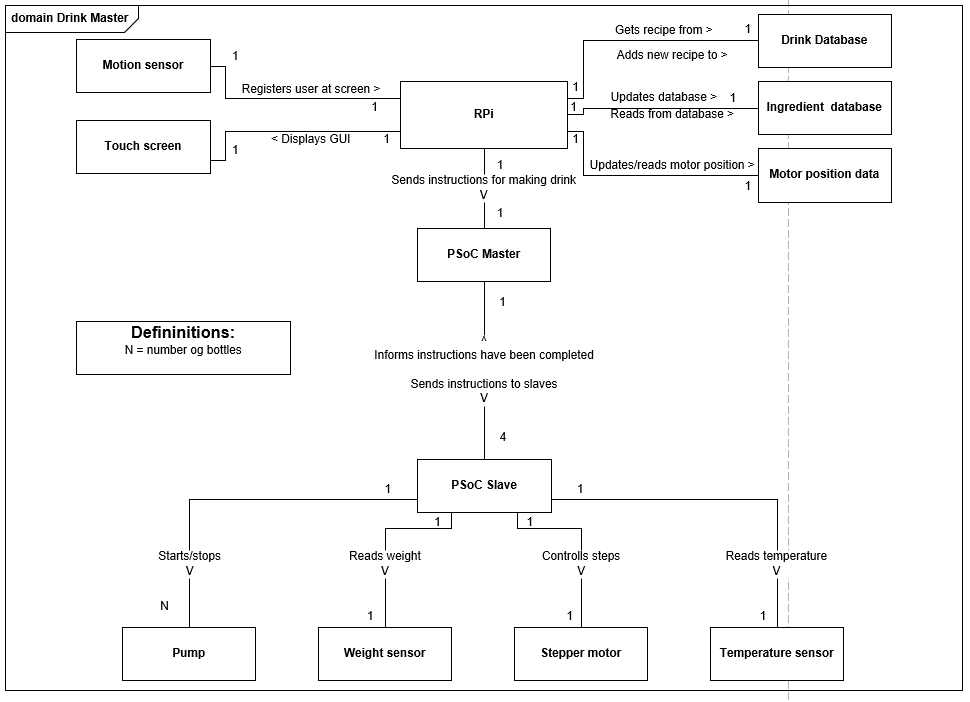
\includegraphics[width=1\textwidth]{Images/domainModel.png}
	\caption{Domæne model for Drink Master}
	\label{fig:domain}
\end{figure}